\pagebreak\section{Introduction}
    \subsection{Arduino}
    Arduino comprises of both a physical programmable circuit board (commonly known as a microcontroller) and a programming software, or IDE (Integrated Development Environment) that can be run
    on a PC, used to compose and transfer PC code to the circuit board. It can be done by using the
    Arduino programming language (based on Wiring), and the Arduino Software (IDE), based on Processing. Unlike other programmable circuit boards, the Arduino does not require a different equipment
    (called a software engineer) to upload code to the circuit board, one can essentially utilize a USB link.
    Also, the Arduino IDE utilizes a rearranged rendition of C++, making it simpler to figure out how
    to program. In a word, Arduino make the functions of the micro-controller into a more accessible
    package. The Uno is one of the more prevalent boards in the Arduino family and an extraordinary
    option for the beginners.
    
    \subsection{Components of the Arduino UNO R3 Board}
    There are different types of Arduino boards for different purposes. But all the boards have the majority of the following components in common. We are going to use an Arduino UNO R3 board for all of our projects.
      
            \begin{center}
                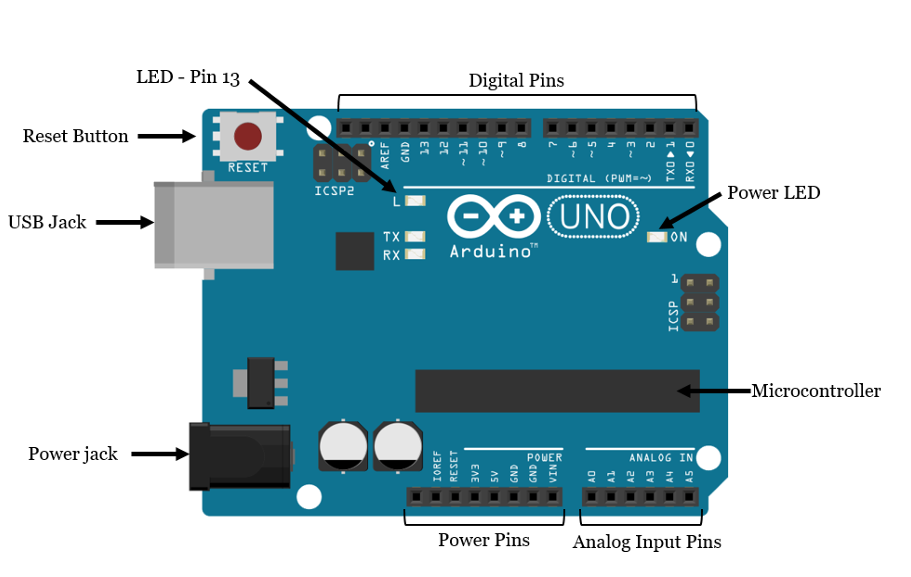
\includegraphics[width =0.8\textwidth]{ArduinoBoard.png}
            \end{center}
      
    
    Starting clockwise from the top center:
    \begin{itemize}
    \item Analog Reference pin (orange)
    \item Digital Ground (light green)
    \item Digital Pins 2-13 (green)
    \item Digital Pins 0-1/Serial In/Out - TX/RX (dark green
    \item  Reset Button - S1 (dark blue)
    \item  In-circuit Serial Programmer (blue-green)
    \item  Analog In Pins 0-5 (light blue)
    \item  Power and Ground Pins (power: orange, grounds: light orange)
    \item  External Power Supply In (9-12VDC) - X1 (pink)
    \item  Toggles External Power and USB Power (place jumper on two pins closest to desired supply) -
    SV1 (purple)
    \item  USB (used for uploading sketches to the board and for serial communication between the board
    and the computer; can be used to power the board) (yellow)
    \end{itemize}
    
    \par- These pins cannot be used for digital i/o (digitalRead and digitalWrite) if serial communication is also being used (e.g. Serial.begin).
        \subsubsection{Digital Pins}
        The digital pins on an Arduino board can be used for general purpose input and output via the pinMode(), digitalRead(), and digitalWrite() commands. Each pin has an internal pull-up resistor which
        can be turned on and off using digitalWrite() (w/ a value of HIGH or LOW, respectively) when the
        pin is configured as an input.
        \begin{itemize}
        \item Serial: 0 (RX) and 1 (TX). Used to receive (RX) and transmit (TX) TTL serial data.[1]
        \item External Interrupts: 2 and 3. These pins can be configured to trigger an interrupt on a low
        value, a rising or falling edge, or a change in value.
        \item PWM: 3, 5, 6, 9, 10, and 11. Provide 8-bit PWM output with the analogWrite() function. On
        boards with an ATmega8, PWM output is available only on pins 9, 10, and 11
        \end{itemize}
    
        \subsubsection{Analog Pins}
        The analog input pins support 10-bit analog-to-digital conversion (ADC) using the analogRead()
        function. Most of the analog inputs can also be used as digital pins: analog input 0 as digital pin 14
        through analog input 5 as digital pin 19.

        \subsubsection{Power Pins}
        \begin{itemize}
            \item \textbf{9V:} The input voltage to the Arduino board when it’s using an external power source (as opposed
            to 5 volts from the USB connection or other regulated power source). Different boards accept
            different input voltages ranges.
            \item \textbf{5V:} The regulated power supply used to power the microcontroller and other components on
            the board. This can come either from VIN via an on-board regulator, or be supplied by USB or
            another regulated 5V supply.
            \item \textbf{3.3V:} (Diecimila-only) A 3.3 volt supply generated by the on-board FTDI chip. 
                \item \textbf{GND:} Ground pins.
        \end{itemize}
        
        
    




